\begin{pastexam}[label={px:ncu-108-dsa-10}]{中央資工所 108 學年度 第 10 題}
（複選；每題 5 分，答錯倒扣 1 分）

Given a weighted undirected graph $G = (V, E)$, let $\delta[u, v]$ denote the distance (the length
of a shortest path) from vertex $u$ to vertex $v$. A path $[v_1, v_2, \ldots, v_k]$ is said to be a
\textit{progress path}, if $\delta[v_i, v_k] > \delta[v_{i+1}, v_k]$ for $1 \le i < k$. For example,
consider the graph with vertex set \{1, 2, 3, 4\} and edge set: (1,2,2), (2,4,1), (3,1,2), (3,4,2),
(1,4,3), where each triple $(i, j, t)$ represents there is an undirected edge between $i$ and $j$
with weight $t$. Then, in this graph, there are totally 2 shortest paths from 1 to 4 (i.e. [1,2,4]
and [1,4]) and there are 3 progress paths from 1 to 4 (they are [1,2,4], [1,4] and [1,3,4]). Now
consider another graph with vertex set \{a, b, c, d, e, f, g, h\} and edge set: (a,b,3), (a,c,1),
(b,c,1), (b,e,5), (b,f,4), (c,d,9), (d,e,5), (d,g,3), (e,f,2), (e,g,2), (f,h,7), (g,h,4). According to this graph, choose the correct item(s):
\begin{enumerate}[label=(\Alph*)]
\item $\delta$[a,h] = 13
\item $\delta$[b,h] = 12
\item $\delta$[d,h] = 6
\item $\delta$[e,h] = 5
\item $\delta$[f,h] = 7
\end{enumerate}
\end{pastexam}

\begin{pastsoln}
答案：(A)(E)。

五個選項問的都是到 h 的距離。 圖是無向圖，$\delta[v, h] = \delta[h, v]$，邊權都是正的，從 h 做一次 Dijkstra
（資結書第~25.2~節）就得到所有點到 h 的距離。 下圖是題目的圖，點旁邊的灰色數字是算出來的 $\delta[\,\cdot\,, h]$。
\begin{center}
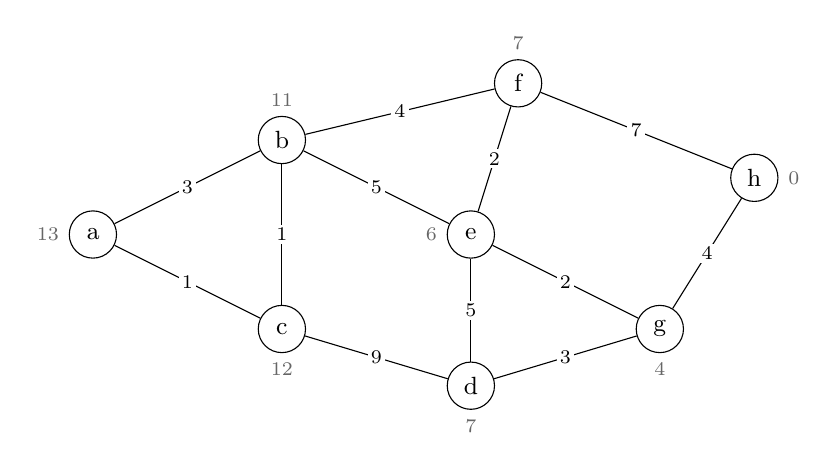
\begin{tikzpicture}[x=1.2cm,y=1.2cm,v/.style={circle,draw,inner sep=0pt,minimum size=6mm,font=\small},
  w/.style={fill=white,inner sep=1.2pt,font=\scriptsize},
  dl/.style={font=\scriptsize,text=black!60}]
\node[v,label={[dl]left:13}] (a) at (0,1) {a};
\node[v,label={[dl]above:11}] (b) at (2,2) {b};
\node[v,label={[dl]below:12}] (c) at (2,0) {c};
\node[v,label={[dl]above:7}] (f) at (4.5,2.6) {f};
\node[v,label={[dl]left:6}] (e) at (4,1) {e};
\node[v,label={[dl]below:7}] (d) at (4,-0.6) {d};
\node[v,label={[dl]below:4}] (g) at (6,0) {g};
\node[v,label={[dl]right:0}] (h) at (7,1.6) {h};
\draw (a)--node[w]{3}(b); \draw (a)--node[w]{1}(c); \draw (b)--node[w]{1}(c);
\draw (b)--node[w]{5}(e); \draw (b)--node[w]{4}(f); \draw (c)--node[w]{9}(d);
\draw (d)--node[w]{5}(e); \draw (d)--node[w]{3}(g); \draw (e)--node[w]{2}(f);
\draw (e)--node[w]{2}(g); \draw (f)--node[w]{7}(h); \draw (g)--node[w]{4}(h);
\end{tikzpicture}
\end{center}
Dijkstra 的過程（每一步取出目前距離最小、還沒確定的點，鬆弛它的邊）：
\begin{center}
\small
\begin{tabular}{clll}
\toprule
步驟 & 取出 & 鬆弛後有變的距離 & 沒有變的 \\
\midrule
1 & h（$0$） & g $= 4$，f $= 7$ & \\
2 & g（$4$） & d $= 4 + 3 = 7$，e $= 4 + 2 = 6$ & \\
3 & e（$6$） & b $= 6 + 5 = 11$ & d：$6 + 5 = 11 > 7$；f：$6 + 2 = 8 > 7$ \\
4 & d（$7$） & c $= 7 + 9 = 16$ & \\
5 & f（$7$） & & b：$7 + 4 = 11$，相同 \\
6 & b（$11$） & c $= 11 + 1 = 12$，a $= 11 + 3 = 14$ & \\
7 & c（$12$） & a $= 12 + 1 = 13$ & \\
8 & a（$13$） & & \\
\bottomrule
\end{tabular}
\end{center}
（第 4、5 步 d、f 的距離都是 $7$，先取哪一個結果都一樣。）

結果：$\delta[\cdot, h]$ 依 a, b, c, d, e, f, g, h 是 $13, 11, 12, 7, 6, 7, 4, 0$。

逐項：
\begin{itemize}
\item (A) $\delta[a,h] = 13$：a--c--b--e--g--h（$1 + 1 + 5 + 2 + 4$）或 a--c--b--f--h（$1 + 1 + 4 + 7$），對。
\item (B) $\delta[b,h] = 11$，不是 $12$，錯。
\item (C) $\delta[d,h] = 7$（d--g--h），不是 $6$，錯。
\item (D) $\delta[e,h] = 6$（e--g--h），不是 $5$，錯。
\item (E) $\delta[f,h] = 7$：直接的邊 $7$，繞 e、g 是 $2 + 2 + 4 = 8$，對。
\end{itemize}
\end{pastsoln}
